\documentclass[conference]{IEEEtran}
\IEEEoverridecommandlockouts
\usepackage{cite}
\usepackage{amsmath,amssymb,amsfonts}
\usepackage{algorithmic}
\usepackage{graphicx}
\usepackage{textcomp}
\usepackage{xcolor}
\usepackage{tabularx}
\usepackage{booktabs}
\usepackage{float}
\usepackage{lipsum}

\def\BibTeX{{\rm B\kern-.05em{\sc i\kern-.025em b}\kern-.08em
    T\kern-.1667em\lower.7ex\hbox{E}\kern-.125emX}}
\begin{document}

\title{Software Requirements Specification \\ for \\ Full-stack based flood risk prediction \\ using ML, DL and QML}

\author{\IEEEauthorblockN{Prepared by:\\

AMMOGH ASHOK\\
LAHARI PANDITH M}
\vspace{0.2cm}
\IEEEauthorblockA{\textit{RV University} \\
Date: 13.03.2026 \\}
}

\maketitle

\tableofcontents
\newpage

\begin{abstract}
This Software Requirements Specification (SRS) outlines the architectural, functional, and non-functional requirements of the Hybrid Flood Risk Prediction System. The proposed system integrates Classical Machine Learning (ML), Deep Learning (DL), and Quantum Machine Learning (QML) paradigms to deliver highly accurate flood risk assessments. The document specifies the user interface, modeling components, data flows, and performance constraints to ensure a robust, scalable, and secure deployment. Furthermore, it details the theoretical frameworks underpinning the Random Forest, Convolutional Neural Networks, and Variational Quantum Classifiers utilized in this ensemble architecture.
\end{abstract}

\section{Introduction}
\subsection{Purpose and scope of srs}
This document delineates the operational parameters and technical specifications for the Hybrid Flood Risk Prediction System. The primary objective of the software is to accurately evaluate the probability of flood events by analyzing a combination of tabular environmental metrics (e.g., rainfall, humidity, temperature, and river levels) and visual satellite or CCTV imagery. The application employs three distinct predictive algorithms: Random Forest for classical machine learning, a Convolutional Neural Network (CNN) for deep learning, and a Variational Quantum Classifier (VQC) via Qiskit for quantum machine learning. A web-based dashboard provides users with an accessible platform to input data, view independent model inferences, and receive a definitive hybrid risk assessment. This SRS acts as a foundational blueprint for developers, project managers, and quality assurance teams to ensure alignment with system objectives.

The necessity of this system arises from the increasing unpredictability of global weather patterns, exacerbated by climate change. Traditional hydrological models often rely on deterministic physics-based simulations that, while accurate, are computationally expensive and struggle to process unstructured data such as satellite imagery in real time. Conversely, purely data-driven machine learning models can struggle with the highly non-linear nature of extreme weather events. By synthesizing classical ensemble methods, deep spatial feature extraction, and the high-dimensional mapping capabilities of quantum circuits, this project aims to create a more resilient and universally applicable early warning system.

\subsection{Document Conventions}
This specification adheres to standardized IEEE formatting conventions. Section headers are clearly marked with Roman numerals, and subsections are alphabetically indexed. Boldface typography highlights critical terminology, while bulleted lists are utilized for outlining specific requirements and constraints. 
\textbf{Abbreviations and Acronyms:}
\begin{itemize}
    \item \textbf{SRS}: Software Requirements Specification
    \item \textbf{ML}: Machine Learning
    \item \textbf{DL}: Deep Learning
    \item \textbf{QML}: Quantum Machine Learning
    \item \textbf{CNN}: Convolutional Neural Network
    \item \textbf{VQC}: Variational Quantum Classifier
    \item \textbf{UI}: User Interface
    \item \textbf{API}: Application Programming Interface
    \item \textbf{REST}: Representational State Transfer
    \item \textbf{IoT}: Internet of Things
    \item \textbf{CI/CD}: Continuous Integration / Continuous Deployment
\end{itemize}

\subsection{Intended Audience and Reading Suggestions}
The target audience encompasses software engineers, data scientists, quantum computing researchers, system testers, and academic supervisors. Developers should prioritize the Functional Requirements and System Architecture sections, while testers should refer to the Nonfunctional Requirements and Analysis Models. Stakeholders seeking a broad overview are advised to focus on the Introduction and Overall Description. Data Scientists will find the mathematical formulations in the Appendix particularly relevant for tuning hyper-parameters and modifying the quantum ansätze.

\subsection{Product Scope}
The software serves as a comprehensive risk evaluation platform intended for environmental researchers, meteorological agencies, and public safety organizations. It allows operators to input real-time localized data and receive an aggregated prediction. By computing a majority vote across disparate AI methodologies, the system dramatically reduces false negatives and offers a fail-safe analytical tool. Future iterations may include real-time IoT sensor integration, automated cron-jobs for live weather data ingestion, and cloud-native quantum hardware offloading via IBM Quantum Services.

The immediate scope covers the deployment of a fully functioning Streamlit web application, containerized via Docker, and orchestrated via Kubernetes. It includes an automated dummy-data generation module to facilitate rapid prototyping and demonstration without relying on external third-party data APIs.

\subsection{References}
\begin{itemize}
    \item IEEE Std 830-1998, IEEE Recommended Practice for Software Requirements Specifications.
    \item Qiskit Machine Learning Documentation (IBM).
    \item PyTorch Vision framework specifications.
    \item Scikit-Learn user guide.
    \item Streamlit API Reference.
    \item Kubernetes Deployment Specifications.
\end{itemize}

\section{Overall Description}
\subsection{Product Perspective}
The Hybrid Flood Risk Prediction System is a standalone web application. It features a responsive frontend developed using the Streamlit library, directly integrated with a Python-based backend. The backend manages data sanitization, model serialization, and inference coordination. The entire application is containerized utilizing Docker, rendering it natively deployable to cloud-based Kubernetes clusters for scalable operation.

The architectural perspective is designed around a microservices-adjacent monolith, where model inference scripts (\texttt{ml\_model.py}, \texttt{dl\_model.py}, \texttt{qml\_model.py}) act as independent utility modules called by the main controller (\texttt{app.py}). This decoupling allows for future isolation of the models into independent microservices accessible via REST APIs.

\subsection{Product Functions}
The application executes the following core operations:
\begin{itemize}
    \item Accepts continuous numerical inputs via interactive UI sliders for localized weather conditions.
    \item Parses and temporarily stores uploaded visual data (JPG/PNG) representing satellite imagery.
    \item Automatically synthesizes baseline dummy datasets for immediate local deployment and model training.
    \item Processes tabular inputs through a trained Random Forest classifier.
    \item Evaluates image data using a PyTorch-based Convolutional Neural Network.
    \item Executes a quantum circuit simulation via Qiskit to derive a Quantum Machine Learning prediction.
    \item Calculates a weighted or unweighted majority vote to formulate the final risk alert.
\end{itemize}

\subsection{User Classes and Characteristics}
\begin{itemize}
    \item \textbf{Meteorological Analysts}: Professionals who possess domain knowledge and require rapid computational models to verify emerging environmental threats. They interact with the system to cross-reference their own meteorological models.
    \item \textbf{General End-Users}: Individuals seeking risk assessments for their immediate geographic locale based on observable data. They require a frictionless UI and clear binary outputs (Flood / No Flood).
    \item \textbf{System Administrators}: Technical personnel tasked with managing Docker containers, maintaining uptime, and optimizing quantum simulator resources. They interact with the Kubernetes deployment files and CI/CD pipelines.
\end{itemize}

\subsection{Operating Environment}
The application requires a standard Python 3.10+ runtime environment. The frontend is accessible via any modern HTML5-compliant web browser. Backend models depend heavily on mathematical computation libraries, including NumPy, Pandas, Scikit-learn, PyTorch, and Qiskit. The hosting machine must possess sufficient RAM to effectively cache the quantum models in memory and prevent disk-serialization errors. A minimum of 8GB of RAM and a multi-core processor are highly recommended to accelerate the state-vector simulations inherent in the Qiskit framework.

\subsection{Design and Implementation Constraints}
\begin{itemize}
    \item \textbf{Computational Overhead}: Quantum Machine Learning simulations are inherently resource-intensive; the training phase is strictly capped at 40 iterations over 100 samples to prevent unacceptable UI latency during initial boot.
    \item \textbf{Serialization Limits}: Due to structural idiosyncrasies in Qiskit 1.0+ and Python's \texttt{pickle} implementation with dynamically generated local functions, models must be persisted in active global RAM rather than serialized to local storage.
    \item \textbf{Storage Limitations}: Image processing is constrained to 64x64 pixel matrices to ensure prompt DL inference times and prevent memory exhaustion on edge devices.
\end{itemize}

\subsection{User Documentation}
Comprehensive setup guidelines, Kubernetes orchestration scripts, and Docker initialization commands are documented within the primary \texttt{README.md} file included in the repository root. This documentation covers local \texttt{pip} installation, containerized execution, and Kubernetes pod deployment strategies.

\subsection{Assumptions and Dependencies}
It is assumed that the host server provides adequate CPU resources for multi-threaded quantum simulations. The system heavily relies on open-source repositories; thus, strict dependency versioning (as outlined in \texttt{requirements.txt}) must be observed to prevent algorithmic deprecation errors. It is also assumed that the end user has a stable internet connection to interact with the Streamlit frontend.

\section{External Interface Requirements}
\subsection{User Interfaces}
The graphical interface is divided into a dual-column layout. The left column captures tabular environmental metrics, while the right column handles image upload functionality. A primary action button executes the inference pipeline. Results are displayed horizontally across three distinct metrics cards, followed by a prominent alert banner denoting the final hybrid decision.

The UI incorporates dynamic visual feedback, utilizing Streamlit's native spinner components to indicate active background processing during model training and inference. Success and Error banners are utilized to color-code the final prediction for immediate cognitive recognition.

\subsection{Hardware Interfaces}
The system does not interface directly with proprietary physical hardware, operating purely within application layer virtualization. However, a multi-core processor is highly recommended to accelerate matrix operations within the PyTorch and Qiskit environments. Future iterations aiming to utilize true Quantum Processing Units (QPUs) will require an internet gateway to interface with IBM Quantum Services via an API token.

\subsection{Software Interfaces}
The backend relies on the Streamlit API to bridge user events with Python execution threads. Data is shuttled between components using standard Pandas DataFrames and NumPy arrays.
\begin{itemize}
    \item \textbf{Scikit-learn}: Interfaces for the Random Forest model and standard scalar transformations.
    \item \textbf{PyTorch}: Interfaces for tensor manipulation and Convolutional Neural Network forward passes.
    \item \textbf{Qiskit}: Interfaces for quantum state compilation, parameter optimization (COBYLA), and local simulation.
\end{itemize}

\subsection{Communications Interfaces}
The frontend communicates with the backend over local HTTP (default port 8501). Standard TCP/IP protocols are utilized for remote web access when deployed on a cloud server. Websockets are implicitly utilized by the Streamlit framework to maintain session state and push UI updates asynchronously to the client browser.

\section{System Features}

\subsection{System Feature 1: Tabular Inference (ML and QML)}
\subsubsection{Description and Priority}
This feature processes the core environmental metrics (rainfall, temperature, humidity, river levels) to predict flood risks using classical and quantum algorithms. Priority: High.
\subsubsection{Stimulus/Response Sequences}
User adjusts numerical sliders and clicks the "Predict" button. The system transmits these vectors to the loaded Random Forest and VQC modules. The UI updates to reflect binary predictions (0 or 1).
\subsubsection{Functional Requirements}
\begin{itemize}
    \item The system must normalize the 4-dimensional input vector prior to QML ingestion using a \texttt{StandardScaler}.
    \item The system shall instantiate a \texttt{ZZFeatureMap} for quantum state preparation, mapping classical data into a high-dimensional Hilbert space.
    \item The Random Forest model must consist of at least 100 decision estimators.
\end{itemize}

\subsection{System Feature 2: Visual Inference (DL)}
\subsubsection{Description and Priority}
Analyzes geographical imagery to ascertain visual markers of flooding using a CNN. Priority: Medium.
\subsubsection{Stimulus/Response Sequences}
User uploads an image file via the drag-and-drop interface. The system renders a thumbnail preview. Upon prediction execution, the system resizes the image to 64x64 RGB tensors and executes a forward pass through the PyTorch model.
\subsubsection{Functional Requirements}
\begin{itemize}
    \item The system must validate the file format (JPG/PNG).
    \item The system must transform the image into a 3-channel PyTorch tensor and normalize pixel values.
    \item In the absence of an image, the system must gracefully skip this module and default to a two-model OR logic for the final prediction.
\end{itemize}

\subsection{System Feature 3: Hybrid Aggregation}
\subsubsection{Description and Priority}
The pivotal logic module that synthesizes a final prediction from individual models. Priority: Critical.
\subsubsection{Stimulus/Response Sequences}
The module receives discrete binary votes from the ML, DL, and QML models. It evaluates the sum against a predefined threshold and renders a final success or error banner.
\subsubsection{Functional Requirements}
\begin{itemize}
    \item If all three models are active (image provided), the threshold for a positive alert is a sum $\geq 2$ (Majority Voting).
    \item If the DL model is inactive (no image provided), the threshold for a positive alert is a sum $\geq 1$ (OR Logic).
\end{itemize}

\section{Other Nonfunctional Requirements}
\subsection{Performance Requirements}
The inference pipeline, excluding the initial memory-caching of models, must execute in under 3.0 seconds to maintain an interactive user experience. The initial quantum model training on the simulator may take between 30 and 60 seconds depending on CPU thread availability, but this latency must only occur once per server lifecycle.

\subsection{Safety Requirements}
In cases where only tabular data is provided, the system utilizes a cautious "OR" voting logic. This is a deliberate safety mechanism designed to minimize false negatives in potential disaster scenarios. If either the classical or quantum model detects a risk anomaly, the warning is escalated to the end-user.

\subsection{Security Requirements}
The application prevents cross-site scripting (XSS) and injection vulnerabilities by inherently escaping user inputs through the Streamlit framework. Uploaded media is stored ephemerally in a temporary directory and scrubbed post-inference or when the session resets. The system does not currently require user authentication, negating the risk of compromised credential storage.

\subsection{Software Quality Attributes}
\begin{itemize}
    \item \textbf{Modularity}: The predictive models are decoupled into discrete Python scripts (\texttt{ml\_model.py}, \texttt{dl\_model.py}, \texttt{qml\_model.py}).
    \item \textbf{Scalability}: Deployment configurations explicitly support container replication via Kubernetes pods (\texttt{k8s-deployment.yaml}).
    \item \textbf{Testability}: A dedicated \texttt{tests/} directory and \texttt{test\_qml.py} script ensure rapid verification of algorithmic modifications.
\end{itemize}

\subsection{Business Rules}
The platform operates as a non-diagnostic advisory tool. Outputs must not be solely relied upon for initiating municipal evacuation protocols without human verification by certified meteorological authorities.

\section{Other Requirements}
Code linting must conform to PEP8 standards, verified by continuous integration pipelines executing Pylint and Pytest. The project includes a pre-configured \texttt{.pylintrc} file to enforce style guidelines and variable naming conventions. Furthermore, GitHub Actions (\texttt{.github/workflows/ci.yml}) are utilized to enforce continuous integration, automatically running tests against all pull requests.

\section*{Appendix A: Glossary}
\begin{itemize}
    \item \textbf{ZZFeatureMap}: A quantum circuit component used to encode classical data into quantum states. It utilizes second-order Pauli-Z rotations to create entanglement between qubits, representing non-linear feature interactions.
    \item \textbf{RealAmplitudes}: A parameterized quantum circuit used as an ansatz in variational algorithms. It consists of alternating layers of parameterized single-qubit Y-rotations and unparameterized CX (CNOT) entangling gates.
    \item \textbf{COBYLA}: Constrained Optimization BY Linear Approximations. A gradient-free optimization algorithm ideal for noisy quantum circuits or simulations where analytical gradients are computationally prohibitive.
    \item \textbf{Majority Voting}: An ensemble machine learning technique where the final class prediction is determined by the class that receives the most votes from the constituent models.
\end{itemize}

\section*{Appendix B: Analysis Models}

\subsection{Data Flow Diagram}
The architecture follows a strict, sequential data flow from ingestion to output. User inputs are serialized by the Streamlit frontend and dispatched to the active models. The QML and ML models receive identical normalized feature vectors, while the DL model receives tensor-transformed image data.

\begin{figure}[H]
\centering
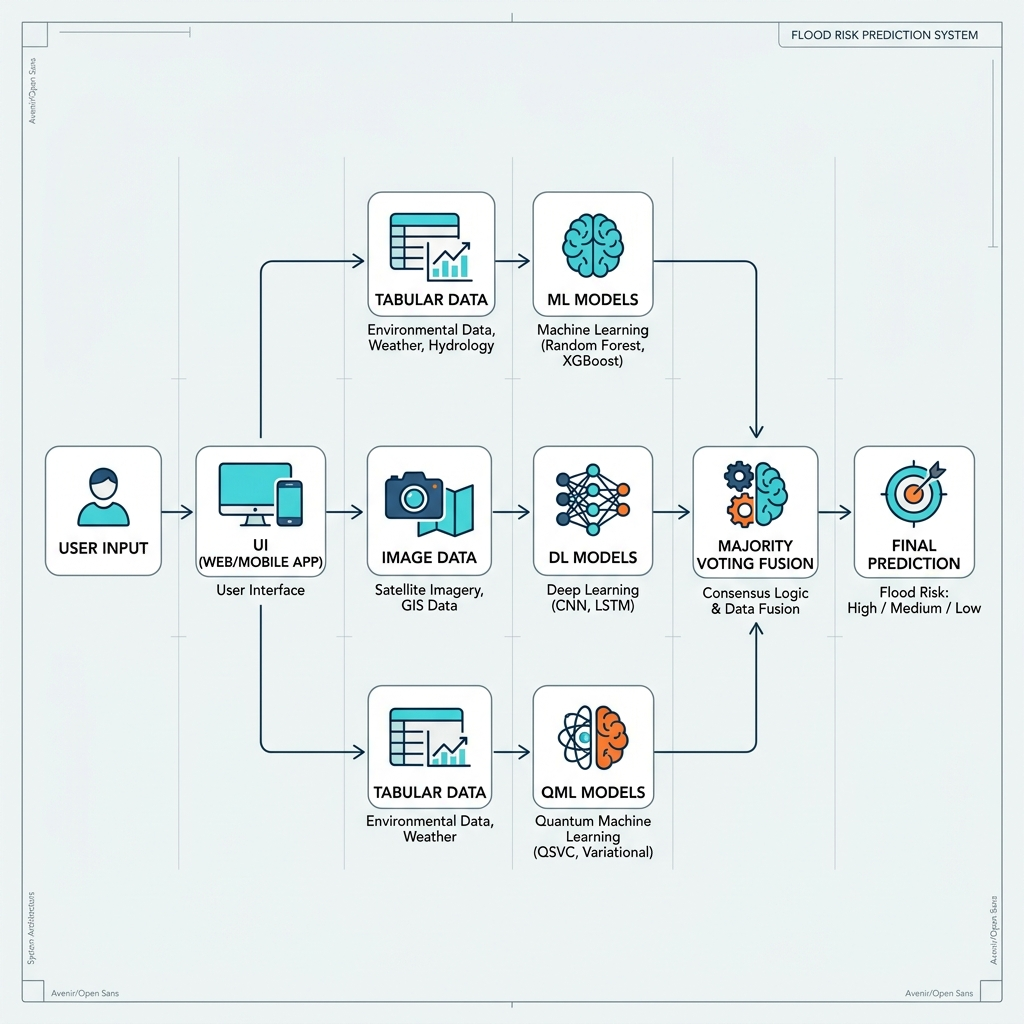
\includegraphics[width=0.45\textwidth]{figures/architecture_dfd.png}
\caption{System Architecture and Data Flow Diagram}
\label{fig:dfd}
\end{figure}

\subsection{UML Use Case Diagram}
The interactions between the end-users and the system components are illustrated below.

\begin{figure}[H]
\centering
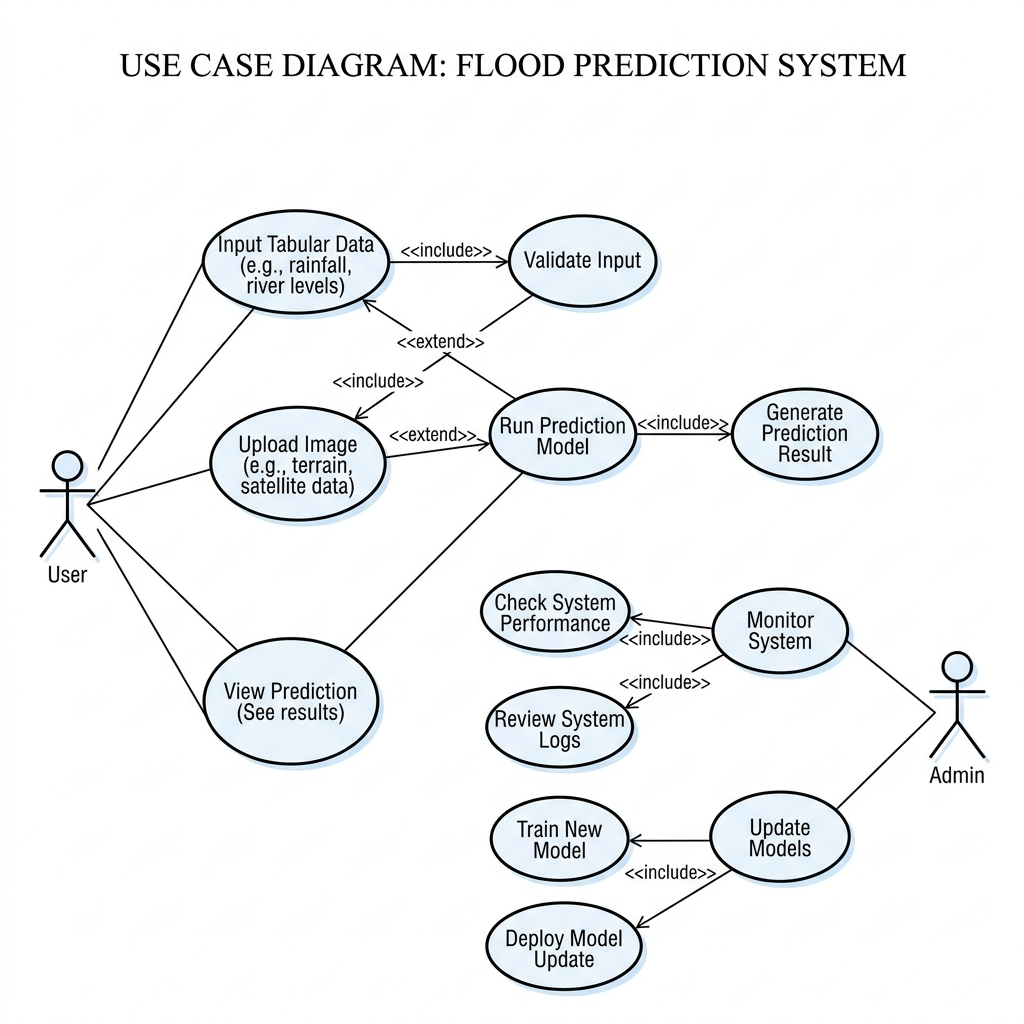
\includegraphics[width=0.45\textwidth]{figures/uml_use_case.png}
\caption{UML Use Case Diagram}
\label{fig:uml}
\end{figure}

\subsection{Entity Relationship Diagram}
Although the current implementation utilizes ephemeral memory and dummy data, the conceptual data structures underpinning the model inferences are structured relationally.

\begin{figure}[H]
\centering
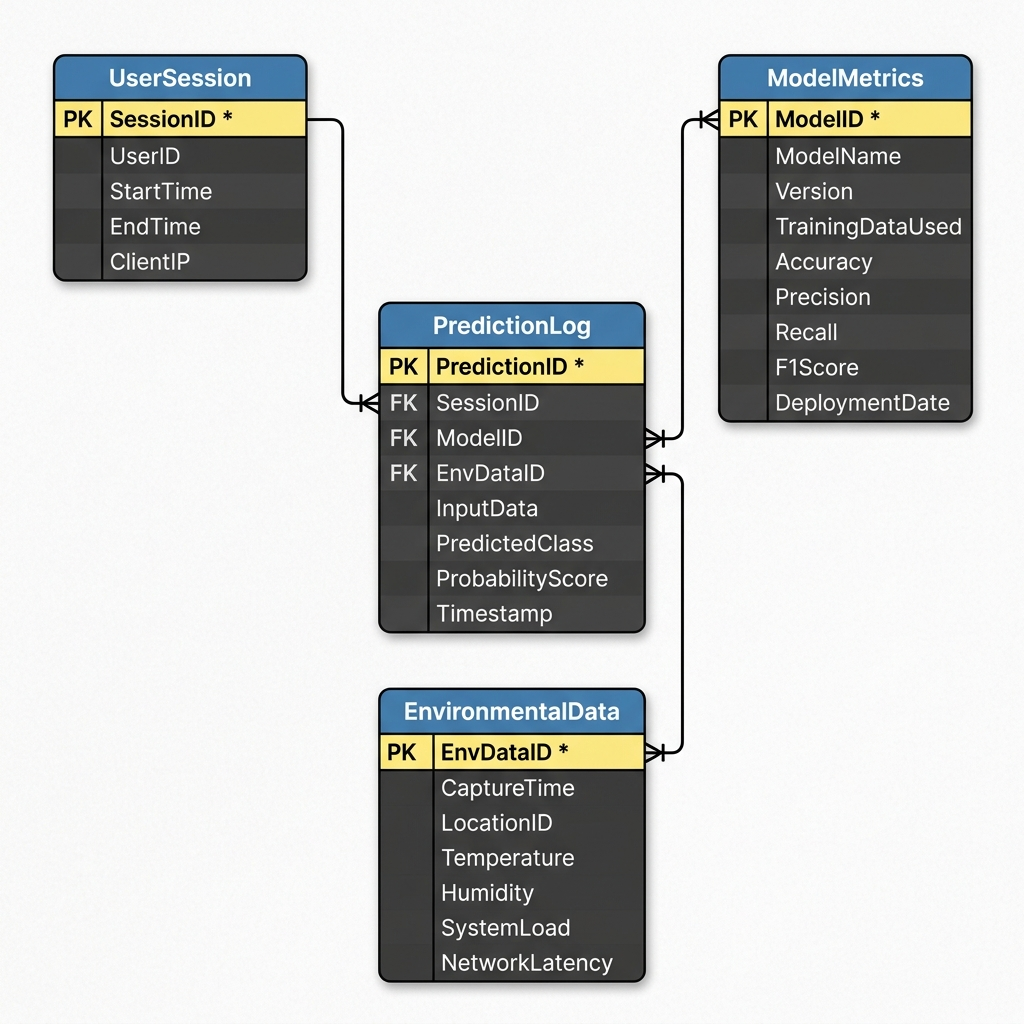
\includegraphics[width=0.45\textwidth]{figures/er_diagram.png}
\caption{Entity Relationship Diagram for Conceptual Data Logging}
\label{fig:er}
\end{figure}

\section*{Appendix C: To Be Determined}
\begin{itemize}
    \item \textbf{External Integrations}: Integration of live external weather APIs (e.g., OpenWeatherMap, NOAA) for automatic tabular data ingestion, overriding the need for manual slider input.
    \item \textbf{Hardware Acceleration}: Optimization of quantum simulations via cloud-based quantum hardware rather than local state-vector simulators. This requires integration with the Qiskit Runtime API.
    \item \textbf{Model Explainability}: Implementation of SHAP (SHapley Additive exPlanations) values to provide users with visual insights into which tabular features (e.g., Rainfall vs. River Level) contributed most significantly to the final prediction.
\end{itemize}

\section*{Appendix D: Mathematical Foundations}

\subsection{Classical Machine Learning (Random Forest)}
The Random Forest algorithm constructs an ensemble of decision trees. For a given input vector $\mathbf{x}$, the final prediction $\hat{y}$ is determined by the mode of the predictions from $B$ individual trees:
\begin{equation}
\hat{y} = \text{mode} \{h_1(\mathbf{x}), h_2(\mathbf{x}), \dots, h_B(\mathbf{x})\}
\end{equation}
where $h_b(\mathbf{x})$ is the prediction of the $b$-th decision tree. Gini impurity is utilized to determine optimal node splits during training:
\begin{equation}
I_G(p) = \sum_{i=1}^{C} p_i (1 - p_i)
\end{equation}

\subsection{Deep Learning (Convolutional Neural Networks)}
The CNN utilizes alternating convolutional and pooling layers to extract hierarchical spatial features from the image tensor. The convolution operation for a 2D image $I$ and a filter $K$ is defined as:
\begin{equation}
(I * K)(i, j) = \sum_{m} \sum_{n} I(i-m, j-n) K(m, n)
\end{equation}
Activation is performed using the Rectified Linear Unit (ReLU) to introduce non-linearity:
\begin{equation}
f(x) = \max(0, x)
\end{equation}
The final classification is produced by a fully connected linear layer mapping the flattened feature maps to binary logits.

\subsection{Quantum Machine Learning (VQC)}
The Variational Quantum Classifier maps classical data $\mathbf{x}$ to a quantum state $|\psi(\mathbf{x})\rangle$ using a feature map $U_{\Phi}(\mathbf{x})$, followed by a parameterized ansatz $W(\boldsymbol{\theta})$. The final state is:
\begin{equation}
|\psi(\mathbf{x}, \boldsymbol{\theta})\rangle = W(\boldsymbol{\theta}) U_{\Phi}(\mathbf{x}) |0\rangle^{\otimes n}
\end{equation}
The prediction is obtained by measuring the parity of the qubit states in the computational basis and assigning the output class based on the highest probability amplitude. The parameters $\boldsymbol{\theta}$ are optimized using the COBYLA algorithm to minimize cross-entropy loss over the training set.

\end{document}
